\documentclass[a4paper]{article}
\usepackage[portuguese]{babel}
\usepackage[utf8]{inputenc}
\usepackage{listings}
\usepackage{graphicx}
\usepackage{float}

\lstset{
numbers=left,
numberstyle=\small,
numbersep=8pt,
language=R,
breaklines=true,
tabsize=4}

\title{Exercício 7 - PCA}

\author{Reconhecimento de Padrões - UFMG}

\date{\small{Guilherme Capanema de Barros (\today)}}

\begin{document}
\maketitle

\section{Introdução}

O método PCA (\textit{Principal Component Analysis}) possibilita a redução da dimensão do problema a ser analisado. Ele faz isso projetando os dados em eixos que seguem as direções de máxima variância, de forma a eliminar dimensões que não oferecem boa separação entre os dados.

Para este trabalho, o método PCA será aplicado em 3 bases de dados: 

\begin{enumerate}
	\item \textbf{BreastCancer}, da biblioteca \textit{mlbanch};
	\item \textbf{USArrests}, nativa do R;
	\item \textbf{Cancer}, da biblioteca \textit{simone}.
\end{enumerate}

Para os itens 1 e 3, a aplicação do PCA será seguida da classificação pelo método SVM.

\section{PCA}

O PCA foi implementado em uma função cujo retorno são os autovetores $\textbf{u}_i$ e os autovalores $\lambda_i$ da matriz de covariâncias do vetor de pontos transladado.

\lstinputlisting{../myPCA.R}

\newpage
\section{Experimentos}

\subsection{BreastCancer}

\subsubsection{PCA}

A base de dados \textit{BreastCancer} possui 9 atributos. A Figura \ref{fig:breastCancerAuto} mostra os autovalores por dimensão PCA e a Figura \ref{fig:breastCancerPlots} mostra os plots bi e tridimensional dos dados.

\begin{figure}[H]
	\centering
	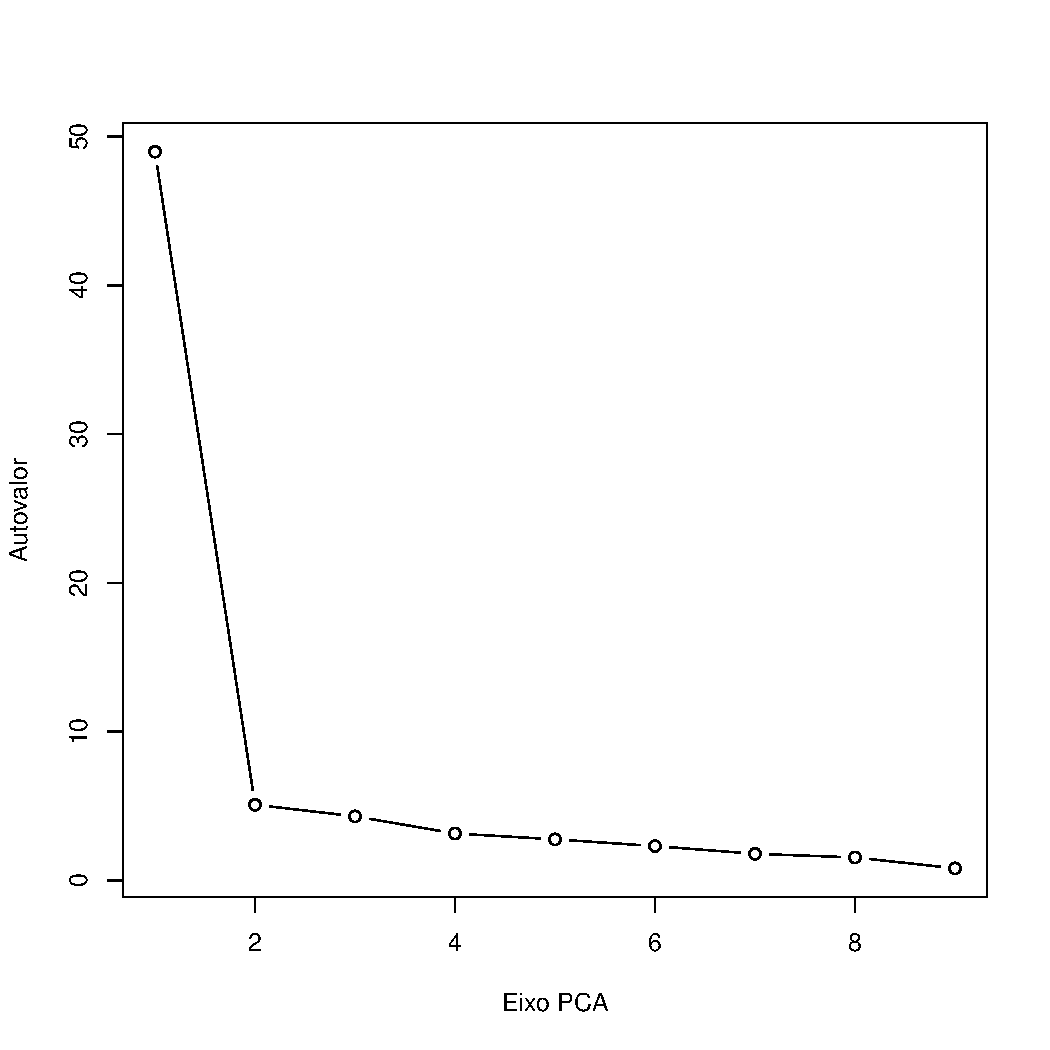
\includegraphics[page=1,width=0.7\textwidth]{../breastCancer.pdf}
	\caption{Autovalores por dimensão para a base de dados \textit{BreastCancer}}
	\label{fig:breastCancerAuto}
\end{figure}

\begin{figure}[H]
	\centering
	\begin{minipage}{.5\textwidth}
		\centering
		\includegraphics[page=2,width=\textwidth]{../breastCancer.pdf}
	\end{minipage}%
	\begin{minipage}{.5\textwidth}
		\centering
		\includegraphics[page=3,width=\textwidth]{../breastCancer.pdf}
	\end{minipage}
	\caption{Plots bidimensional e tridimensional para a base de dados \textit{BreastCancer}}
	\label{fig:breastCancerPlots}
\end{figure}

Abaixo, o código usado para gerar essas visualizações:

\lstinputlisting[firstline=2,lastline=33]{../breastCancer.R}

\subsubsection{Classificação}

Para fins de comparação, o algoritmo SVM desenvolvido em etapass anteriores foi aplicado na base de dados original, bidimensional e tridimensional. Os resultados obtidos estão apresentados na Tabela \ref{tab:breastCancer}.

\begin{table}[H]
	\centering
	\caption{Acurácias do SVM para a base \textit{BreastCancer}}
	\thinspace
	\label{tab:breastCancer}
\begin{tabular}{ c | c | c }
	Original & 2 dimensões & 3 dimensões\\
	\hline
	96,08\% & 93,63\% & 93,63\% \\
\end{tabular}
\end{table}

Abaixo, o código usado para gerar esses dados:

\lstinputlisting[firstline=36,lastline=77]{../breastCancer.R}

\newpage
\subsection{USArrests}

A base de dados \textit{USArrests} possui 4 atributos. A Figura \ref{fig:usArrestsAuto} mostra os autovalores por dimensão PCA e a Figura \ref{fig:usArrestsPlots} mostra os plots bi e tridimensional dos dados.

\begin{figure}[H]
	\centering
	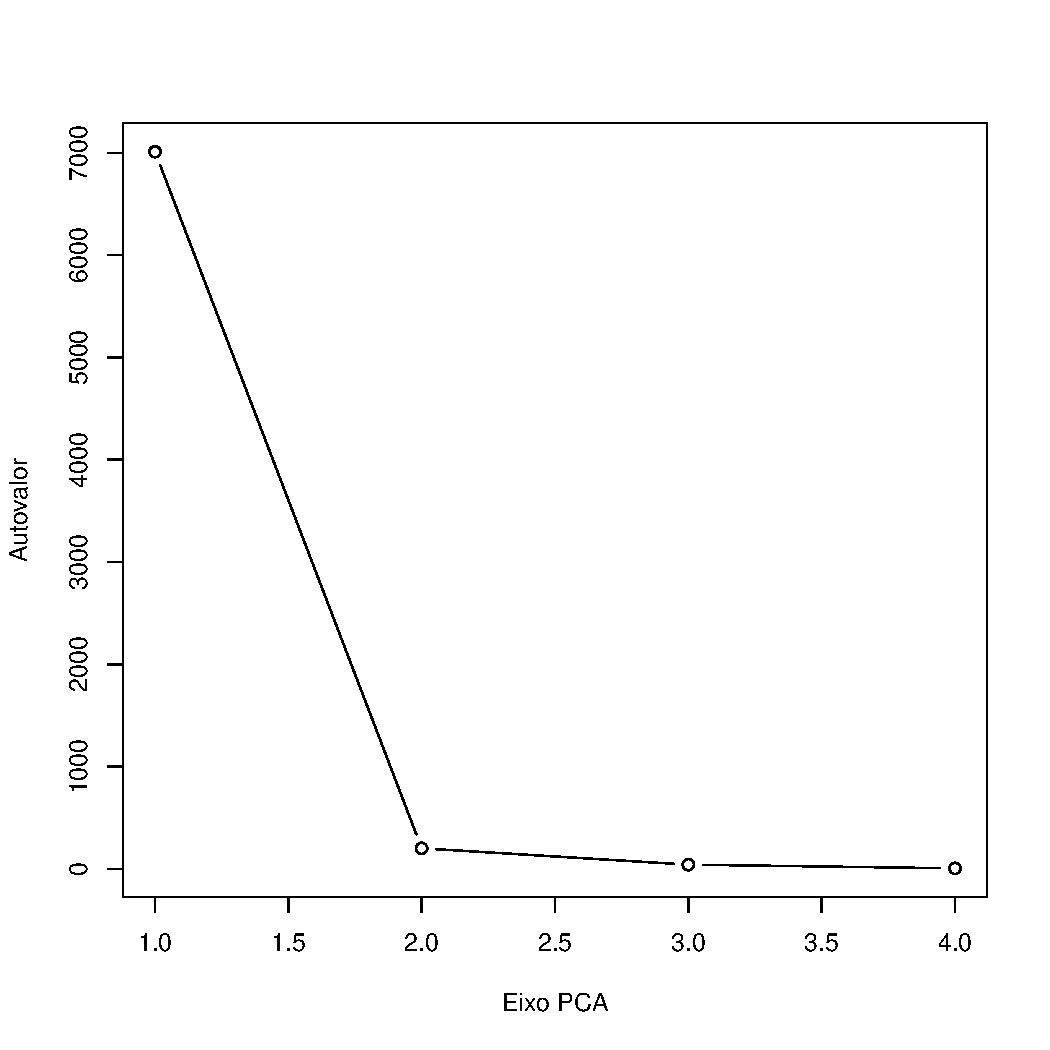
\includegraphics[page=1,width=0.7\textwidth]{../usArrests.pdf}
	\caption{Autovalores por dimensão para a base de dados \textit{USArrests}}
	\label{fig:usArrestsAuto}
\end{figure}

\begin{figure}[H]
	\centering
	\begin{minipage}{.5\textwidth}
		\centering
		\includegraphics[page=2,width=\textwidth]{../usArrests.pdf}
	\end{minipage}%
	\begin{minipage}{.5\textwidth}
		\centering
		\includegraphics[page=3,width=\textwidth]{../usArrests.pdf}
	\end{minipage}
	\caption{Plots bidimensional e tridimensional para a base de dados \textit{USArrests}}
	\label{fig:usArrestsPlots}
\end{figure}

Abaixo, o código usado para gerar essas visualizações:

\lstinputlisting[firstline=2]{../usArrests.R}

\newpage
\subsection{Cancer}

\subsubsection{PCA}

A base de dados \textit{Cancer} possui 26 atributos. A Figura \ref{fig:cancerAuto} mostra os autovalores por dimensão PCA e a Figura \ref{fig:cancerPlots} mostra os plots bi e tridimensional dos dados.

\begin{figure}[H]
	\centering
	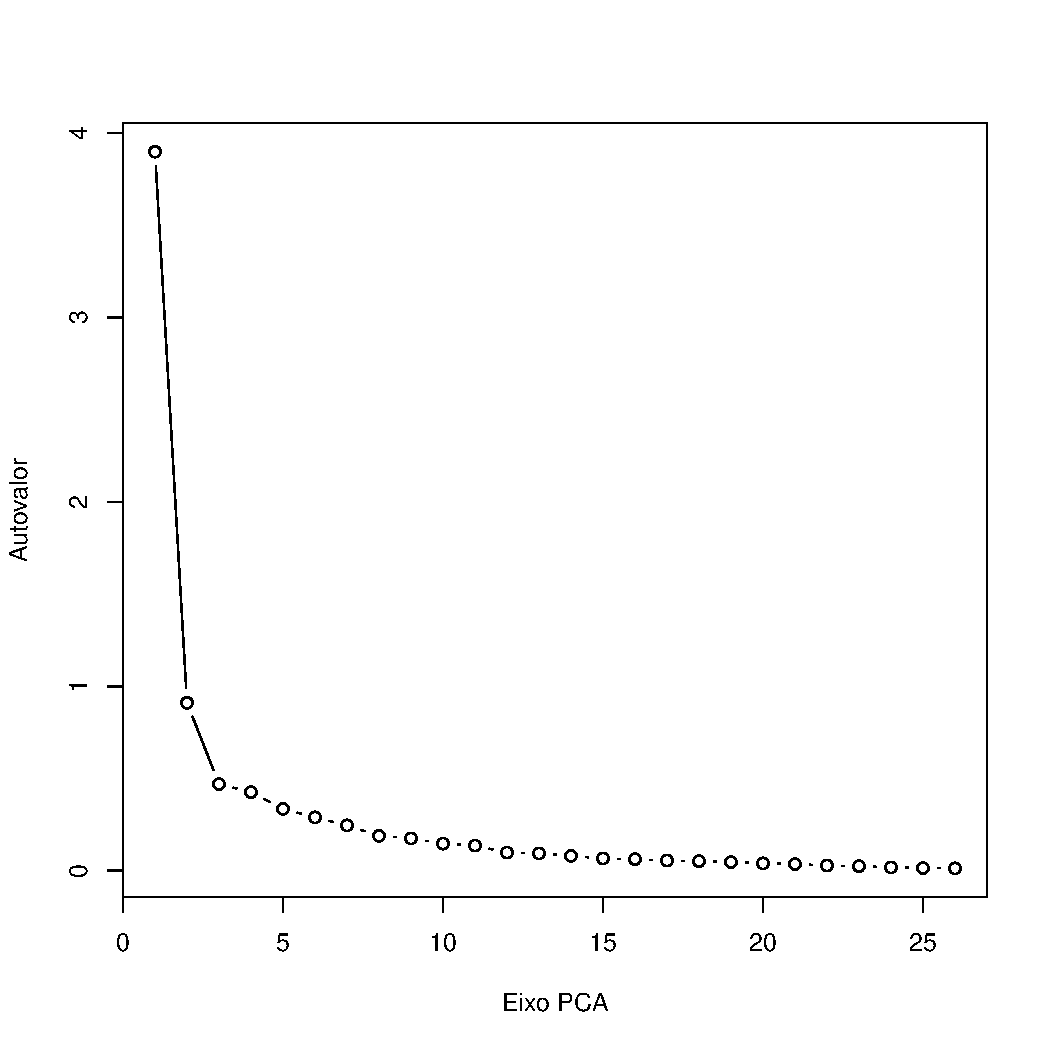
\includegraphics[page=1,width=0.7\textwidth]{../cancer.pdf}
	\caption{Autovalores por dimensão para a base de dados \textit{Cancer}}
	\label{fig:cancerAuto}
\end{figure}

\begin{figure}[H]
	\centering
	\begin{minipage}{.5\textwidth}
		\centering
		\includegraphics[page=2,width=\textwidth]{../cancer.pdf}
	\end{minipage}%
	\begin{minipage}{.5\textwidth}
		\centering
		\includegraphics[page=3,width=\textwidth]{../cancer.pdf}
	\end{minipage}
	\caption{Plots bidimensional e tridimensional para a base de dados \textit{Cancer}}
	\label{fig:cancerPlots}
\end{figure}

Abaixo, o código usado para gerar essas visualizações:

\lstinputlisting[firstline=2,lastline=32]{../cancer.R}

\subsubsection{Classificação}

Para fins de comparação, o algoritmo SVM desenvolvido em etapass anteriores foi aplicado na base de dados original, bidimensional e tridimensional. Os resultados obtidos estão apresentados na Tabela \ref{tab:cancer}.

\begin{table}[H]
	\centering
	\caption{Acurácias do SVM para a base \textit{Cancer}}
	\thinspace
	\label{tab:cancer}
\begin{tabular}{ c | c | c }
	Original & 2 dimensões & 3 dimensões\\
	\hline
	84,62\% & 76,92\% & 72,92\% \\
\end{tabular}
\end{table}

Abaixo, o código usado para gerar esses dados:

\lstinputlisting[firstline=35]{../cancer.R}

\section{Conclusão}

Fica claro que, para as bases de dados analisadas, a aplicação do PCA para redução das dimensões tem baixo impacto na acurácia final dos classificadores. A simplificação dos problemas pode resultar, portanto, em modelos mais rápidos e simples, com baixa perda de acurácia.

\end{document}
